\chapter{Case study and experimental setup}
	L'elaborato è stato condotto sfruttando due sistemi differenti, aventi ruolo di \emph{client} e \emph{server}.\par
	Il client ha un processore \texttt{Intel Celeron N3050} $1.60GHz$,  memoria di $4GB$ ed un sistema operativo \texttt{Ubuntu 18.04.1 LTS}.\par
	Il server è costituito da una macchina virtuale con sistema operativo \texttt{Trisquel-mini 8.0}, distribuzione di \emph{GNU} con kernel \emph{Linux-libre}, memoria di $512GB$, risiedente su un sistema con processore \texttt{Intel Core i3} $2.27GHz$.\par
	Il web server utilizzato è \emph{Apache Web Server} versione 2, il load generator \emph{Apache JMeter 5.0}. Esso consente l'invio di richieste HTTP al server con tasso impostabile. La scelta delle pagine su cui incentrare l'esperimento è stata dettata da una ricerca sul web delle dimensioni di quelle, a nostro parere, maggiormente rappresentative: social network, e-commerce, blog, siti aziendali, wiki. Infine abbiamo sfruttato per la scelta il report di \emph{HTTP Archive} sullo stato del web. Esso, infatti, evidenzia come le pagine web, in contesto desktop e mobile, stiano aumentando di dimensioni, passando dalle centinaia di $KB$, al $MB$.
	\begin{figure}[H]
		\centering
		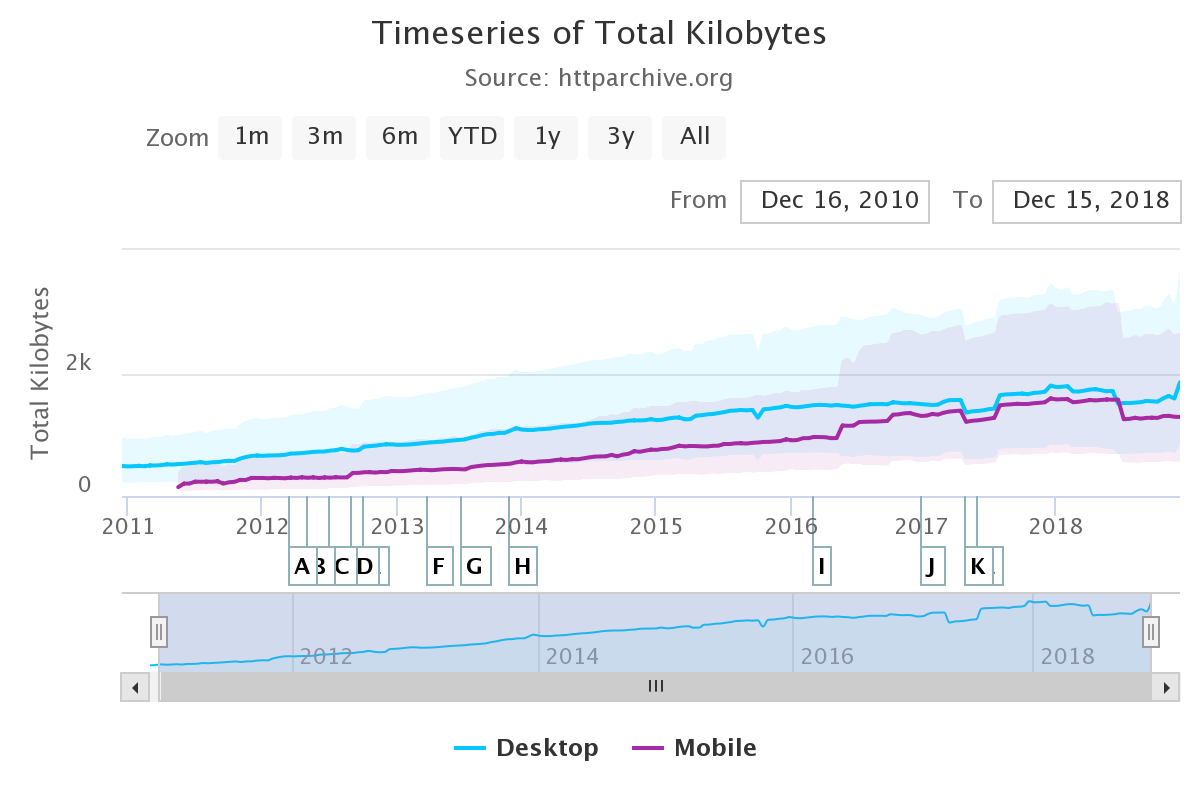
\includegraphics[scale=0.3]{./immagine/chart.png}
		\caption{Stato del Web: Kilobyte totali}
		\label{fig:httparc}
	\end{figure}
	
	\section{Workload Characterization}
		Mediante Jmeter, sono state inviate al server $60req/s$ di 5 diversi tipi di pagine. Il tasso di richieste è stato impostato con il \emph{Constant Throughput Timer}, selezionando $3600req/min$, svolte dai thread complessivamente. Le richieste sono infatti eseguite da 30 thread per 5 minuti. Ogni richiesta può essere casualmente di uno dei 5 tipi:
		\begin{itemize}
			\item \emph{Instagramlogin.html} di $32MB$
			\item \emph{FrancoCFA.html} di $112KB$
			\item \emph{Amazon.html} di $460KB$
			\item \emph{Facebook.html} di $1.4MB$
			\item \emph{Sample-jpg-image-5mb.jpg} di $1MB$
		\end{itemize}
		
		I dati di application level sono stati raccolti con un \emph{Simple Data Writer}. Lato server i dati system level sono stati collezionati per 6 minuti, tramite il comando \textsf{vmstat -n -a 1 360}. Alcune istanze, quindi, tra questi sono precedenti e successive all'esperimento.
	\section{Capacity Test}
		Il Capacity Test è stato eseguito con le pagine Amazon.html, Facebook.html, Sample-jpg-image-5mb.jpg, rappresentanti tipologie di pagine piccole, medie e grandi. Il test è stato attuato prima considerando tutte le pagine (\emph{Random Controller}), poi ciascuna singolarmente.\par
		Throughput e response time sono stati analizzati al crescere delle richieste al minuto. Diverse osservazioni sono state collezionate per una singola condizione di carico, caratterizzate, poi, dalla media, poiché c'è interesse nell'andamento globale.\par
		Il tasso di richieste desiderato è stato ottenuto stabilendo il tasso per ciascun thread ed incrementando ogni volta il loro numero.
		
		\begin{table}
			\footnotesize
			\caption{Capacity Test per tipo di richiesta}
			\label{tab:ct-tip}
			\centering
			\begin{tabular}{cp{0.5\textwidth}c}
				\toprule
				\textbf{Tipo} &
				\textbf{Usable Capacity} &
				\textbf{Knee Capacity}\\
				\midrule
				Random &
				120 &
				50\\
				\midrule
				Piccola &
				600 &
				200\\
				\midrule
				Media &
				220 &
				88\\
				\midrule
				Grande &
				80 &
				20\\
				\bottomrule			
			\end{tabular}
		\end{table}
	
		I risultati ottenuti sono riportati in \textbf{Tabella \ref{tab:ct}}. Di seguito l'andamento di throughput (1/min) e response time (ms), all'aumentare del carico nei 4 casi considerati.
		
		\begin{figure}[H]
			\centering
			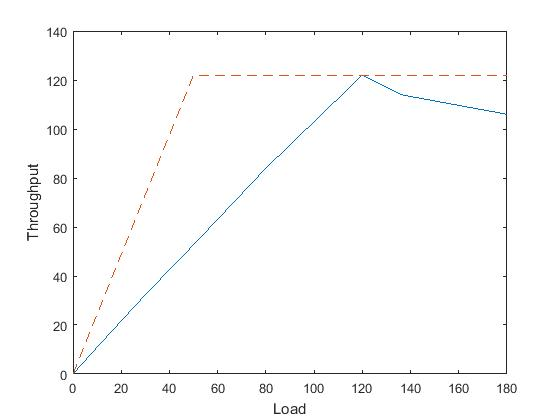
\includegraphics[scale=0.6]{./immagine/randomT.jpg}
			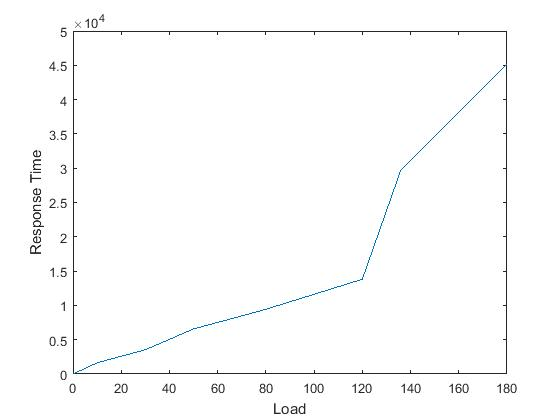
\includegraphics[scale=0.6]{./immagine/randomR.jpg}
			\caption{Pagine Random}
			\label{fig:ct-r}
		\end{figure}
		\begin{figure}[H]
			\centering
			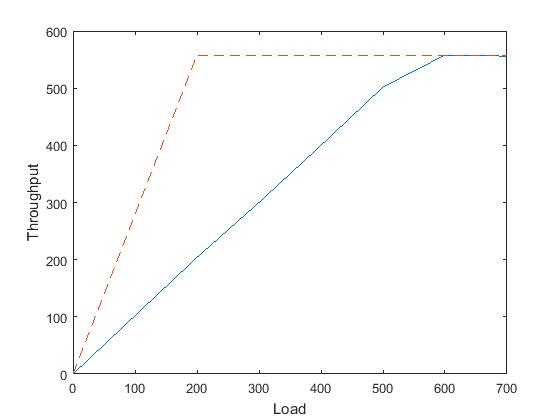
\includegraphics[scale=0.6]{./immagine/piccolaT.jpg}
			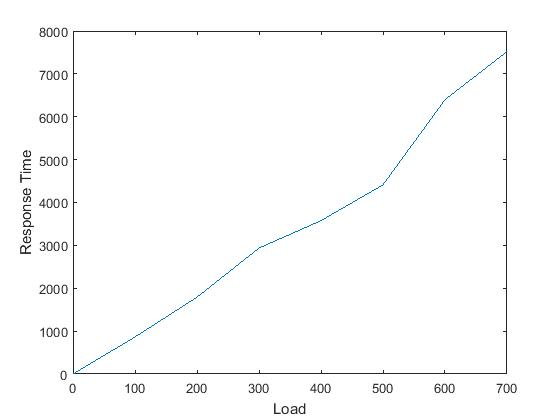
\includegraphics[scale=0.6]{./immagine/piccolaR.jpg}
			\caption{Pagine Piccole}
			\label{fig:ct-p}
		\end{figure}
		\begin{figure}[H]
			\centering
			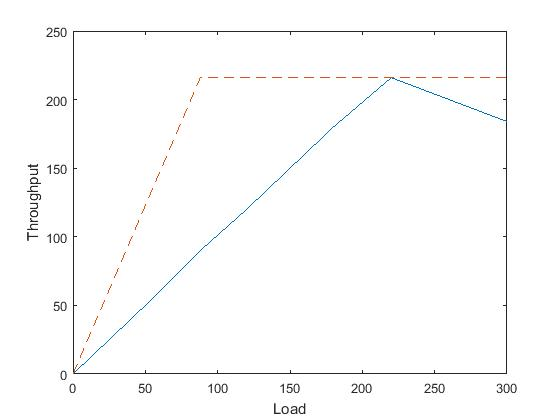
\includegraphics[scale=0.6]{./immagine/mediaT.jpg}
			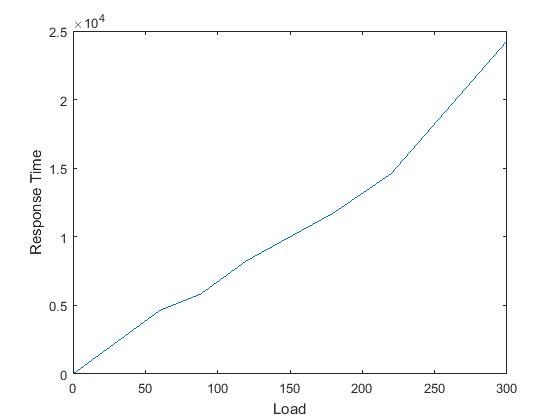
\includegraphics[scale=0.6]{./immagine/mediaR.jpg}
			\caption{Pagine Medie}
			\label{fig:ct-m}
		\end{figure}
		\begin{figure}[H]
			\centering
			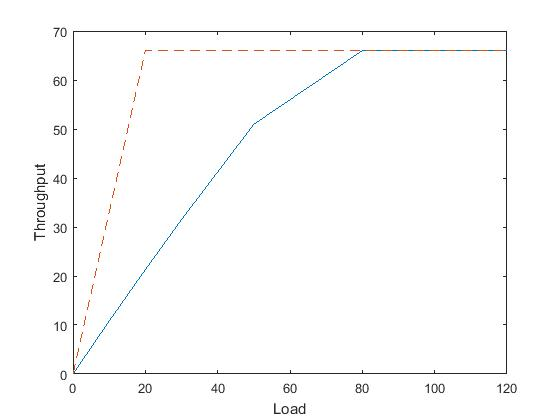
\includegraphics[scale=0.6]{./immagine/grandeT.jpg}
			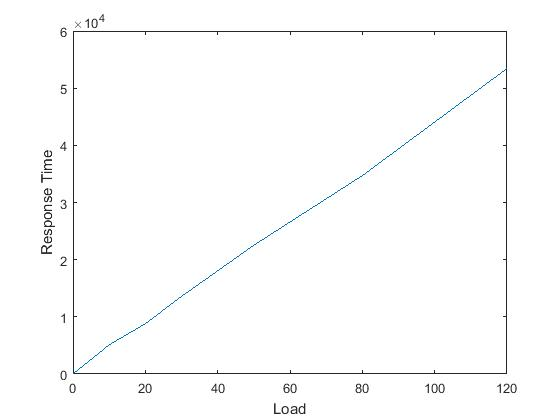
\includegraphics[scale=0.6]{./immagine/grandeR.jpg}
			\caption{Pagine Grandi}
			\label{fig:ct-g}
		\end{figure}
	
		Infine possiamo ricavare i valori per il caso medio ed il caso peggiore delle 3 tipologie di pagine (\textbf{Tabella \ref{tab:ct}}). Osserviamo come il caso medio presenti valori superiori agli altri, poiché molto influenzato dal peso delle pagine piccole. Esse rappresentano la maggioranza delle pagine web di dimensione di centinaia di $KB$, escluse quelle relative ai social network, e non riescono a saturare velocemente il server.
		
		\begin{table}
			\footnotesize
			\caption{Capacity Test}
			\label{tab:ct}
			\centering
			\begin{tabular}{cp{0.5\textwidth}c}
				\toprule
				\textbf{Case} &
				\textbf{Usable Capacity} &
				\textbf{Knee Capacity}\\
				\midrule
				Random &
				120 &
				50\\
				\midrule
				Average &
				300 &
				102.7\\
				\midrule
				Worst &
				80 &
				20\\
				\bottomrule			
			\end{tabular}
		\end{table}
	
	\section{Experimental Design and Analysis}
		Per studiare l'impatto del tasso di richiesta e del tipo di pagina sul tempo di risposta medio, si prosegue con la tecnica del \emph{Design of Experiment}. I fattori sono stati categorizzati. Si sono considerati 2 tipi di pagina: Piccola (Amazon.html), Grande (Sample-jpg-image-5mb.jpg). Si sono poi determinati 4 livelli per il tasso di richiesta, corrispondenti al 20\%, 40\%, 60\%, 80\% della usable capacity media delle pagine: Low, Low-Medium, High-Medium, High. I trattamenti sono stati ripetuti per 10 volte ed in ordine casuale, con durata di 1 minuto ciascuno. Tramite JMP si è ricavata la stima del modello.
		
		\begin{figure}[H]
			\centering
			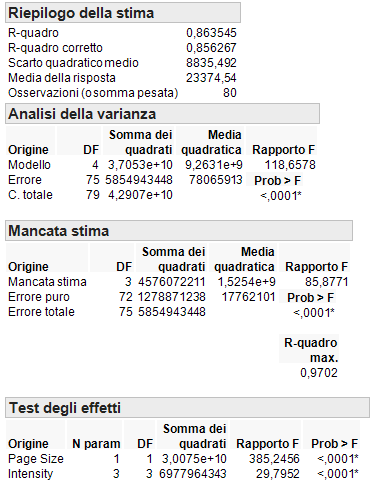
\includegraphics{./immagine/Stimamodello1.png}
			\label{fig:doe-st}
			\caption{Analisi della varianza}
		\end{figure}
	
		Dal rapporto della somma dei quadrati dei fattori rispetto a quella totale, si evince la loro importanza: 70\% della variazione totale è attribuito a Page Size, 16.3\% ad Intensity, il resto all'errore. In realtà parte dell'importanza dell'errore è dovuta all'interazione tra i fattori trascurata, che rappresenta il 10.7\% della variazione totale. Il modello, quindi, spiega circa 86.3\% di SST, come testimonia anche $R^2$.\par
		Per la scelta del tipo di analisi, si provano le assunzioni di normalità ed omoschedasticità. Per la normalità si effetua il \emph{Quantile-Quantile plot} dei residui. Si osserva che la loro distribuzione è asimmetrica. Ciò può essere anche confermato dal test di \emph{Shapiro-Wilk}, che restituisce $p<0.05$, rigettando l'ipotesi di normalità.
		
		\begin{figure}[H]
			\centering
			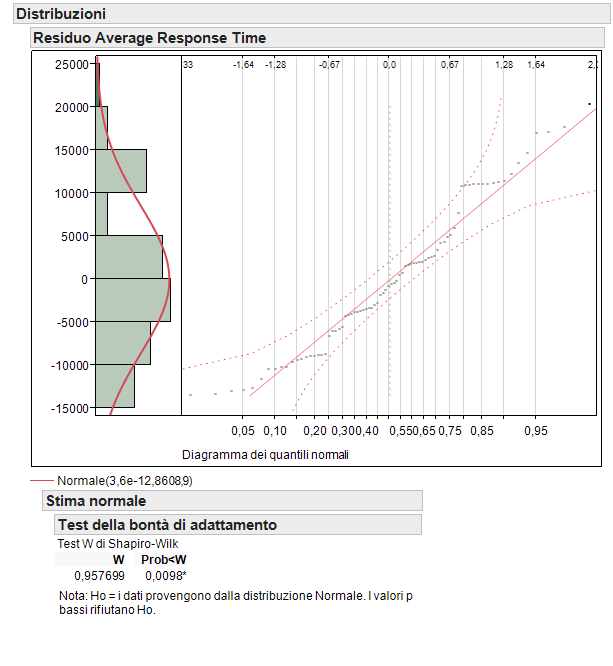
\includegraphics{./immagine/Distribuzione.png}
			\label{fig:doe-n}
			\caption{Q-Q plot e test di Shapiro-Wilk}
		\end{figure}
	
		Necessitiamo, quindi, di un'analisi non parametrica. Ciò può farci già propendere per il test di \emph{Wilcoxon/Kruskal-Wallis}, anche senza valutare l'omoschedasticità (che da test visuale risulta non verificata).
		
		\begin{figure}[H]
			\centering
			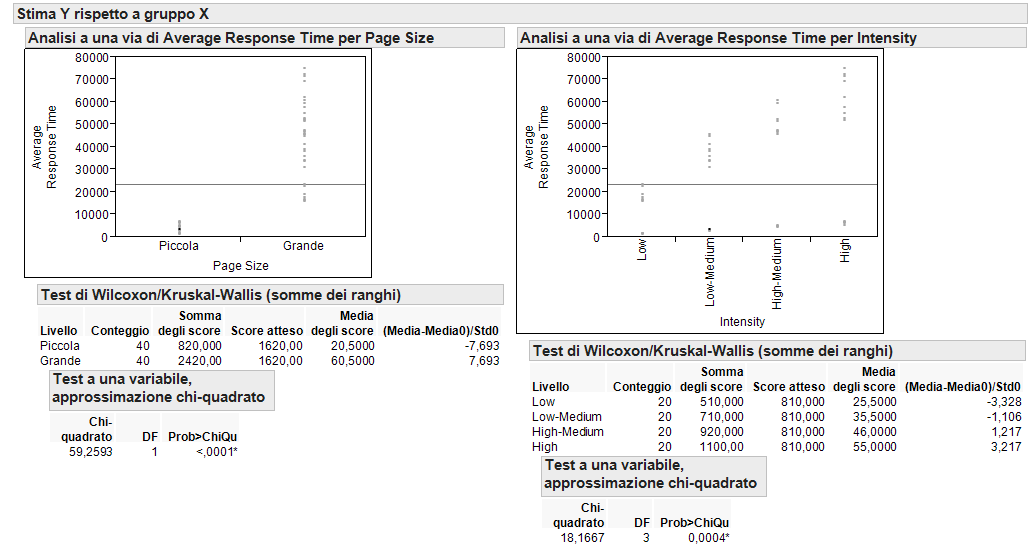
\includegraphics[scale=0.6]{./immagine/StimaYrispettoaX.png}
			\caption{Test di Wilcoxon/Kruskal-Wallis}
			\label{fig:doe-yx}
		\end{figure}
	
		Il test di Kruskal-Wallis rigetta l'ipotesi nulla (campioni dalla stessa popolazione) per entrambi i fattori. Troviamo, infatti, $p<0.05$, quindi entrambi gli effetti sono statisticamente significativi con livello di significatività 0.05.
	